\documentclass[border=6pt]{standalone}
% Shared preamble for web figures.  Each figure is a standalone .tex that
% \input's this file; scripts/make-figures.sh turns it into an SVG.
% Handouts pull the same file with \fig{Unit_X/<name>}.
\usepackage[T1]{fontenc}
\usepackage{helvet}
\renewcommand{\familydefault}{\sfdefault}
\renewcommand{\ttdefault}{pcr}  % Courier: a real Type 1 typewriter font
\usepackage{amsmath}
\usepackage{tikz}
\usetikzlibrary{arrows.meta,positioning,calc,shapes.symbols,shapes.geometric}

% Who makes the rules is the point of most diagrams in this book, so the
% colors mean the same thing everywhere: blue is a person, orange is the
% computer, green is an answer, pink is the human brain.
\definecolor{person}{HTML}{2C6FAE}
\definecolor{machine}{HTML}{D35400}
\definecolor{result}{HTML}{1E8449}
\definecolor{brainpink}{HTML}{C2185B}
\definecolor{ink}{HTML}{2C3E50}

\tikzset{
  doodle/.style={line width=1.5pt, line cap=round, line join=round, draw=ink},
  box/.style={draw, rounded corners=5pt, line width=1.1pt, align=center,
              inner sep=7pt, minimum height=1.0cm, font=\small},
  personbox/.style={box, draw=person, fill=person!10},
  machinebox/.style={box, draw=machine, fill=machine!10},
  resultbox/.style={box, draw=result, fill=result!10},
  plainbox/.style={box, draw=ink!70, fill=ink!4},
  flow/.style={-{Stealth[length=8pt]}, line width=1.4pt, draw=ink},
}

% A person (blue) and a robot head (orange) as small icons.
% \personicon{x}{y}{scale}   \roboticon{x}{y}{scale}
\newcommand{\personicon}[3]{%
  \begin{scope}[shift={(#1,#2)}, scale=#3]
    \fill[person] (0,0.62) circle (0.28);
    \fill[person, rounded corners=6pt] (-0.42,-0.55) rectangle (0.42,0.28);
  \end{scope}}
\newcommand{\roboticon}[3]{%
  \begin{scope}[shift={(#1,#2)}, scale=#3]
    \draw[machine, line width=1.2pt] (0,0.5) -- (0,0.72);
    \fill[machine] (0,0.78) circle (0.08);
    \draw[machine, line width=1.4pt, fill=machine!12, rounded corners=4pt] (-0.5,-0.45) rectangle (0.5,0.5);
    \fill[ink] (-0.2,0.12) circle (0.08);
    \fill[ink] (0.2,0.12) circle (0.08);
    \draw[ink, line width=1pt] (-0.22,-0.22) -- (0.22,-0.22);
  \end{scope}}

\begin{document}
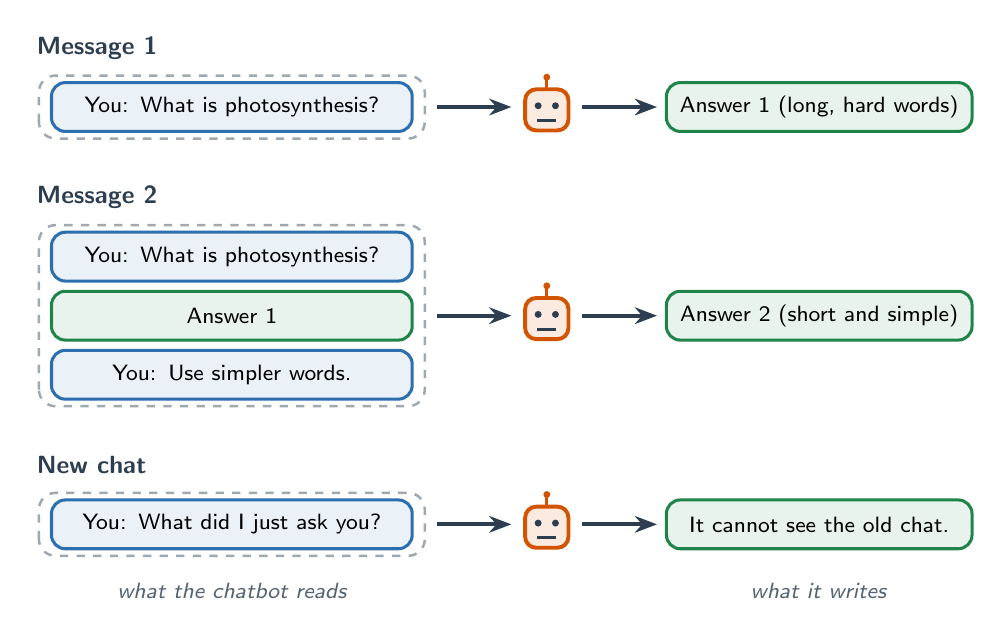
\begin{tikzpicture}[
  msg/.style={box, font=\footnotesize, minimum height=0.62cm, inner sep=4pt, text width=4.3cm},
  you/.style={msg, draw=person, fill=person!10},
  bot/.style={msg, draw=result, fill=result!10},
  stack/.style={draw=ink!45, dashed, rounded corners=6pt, line width=0.9pt},
  head/.style={font=\small\bfseries, text=ink, anchor=west},
]
% Every new message, the chatbot reads the whole chat again from the top.
% Row 1: first message
\node[head] at (-2.6,1.15) {Message 1};
\node[you] (a1) at (0,0.4) {You: What is photosynthesis?};
\draw[stack] (-2.45,0.0) rectangle (2.45,0.8);
\roboticon{4.0}{0.35}{0.55}
\draw[flow] (2.6,0.4) -- (3.55,0.4);
\draw[flow] (4.45,0.4) -- (5.4,0.4);
\node[bot, text width=3.6cm, anchor=west] at (5.5,0.4) {Answer 1 (long, hard words)};

% Row 2: follow-up
\node[head] at (-2.6,-0.75) {Message 2};
\node[you] (b1) at (0,-1.5) {You: What is photosynthesis?};
\node[bot] (b2) at (0,-2.25) {Answer 1};
\node[you] (b3) at (0,-3.0) {You: Use simpler words.};
\draw[stack] (-2.45,-3.4) rectangle (2.45,-1.1);
\roboticon{4.0}{-2.3}{0.55}
\draw[flow] (2.6,-2.25) -- (3.55,-2.25);
\draw[flow] (4.45,-2.25) -- (5.4,-2.25);
\node[bot, text width=3.6cm, anchor=west] at (5.5,-2.25) {Answer 2 (short and simple)};

% Row 3: new chat
\node[head] at (-2.6,-4.15) {New chat};
\node[you] (c1) at (0,-4.9) {You: What did I just ask you?};
\draw[stack] (-2.45,-5.3) rectangle (2.45,-4.5);
\roboticon{4.0}{-4.95}{0.55}
\draw[flow] (2.6,-4.9) -- (3.55,-4.9);
\draw[flow] (4.45,-4.9) -- (5.4,-4.9);
\node[bot, text width=3.6cm, anchor=west] at (5.5,-4.9) {It cannot see the old chat.};

\node[font=\footnotesize\itshape, text=ink!80, align=center] at (0,-5.75) {what the chatbot reads};
\node[font=\footnotesize\itshape, text=ink!80, align=center] at (7.45,-5.75) {what it writes};
\end{tikzpicture}
\end{document}
